\usetikzlibrary{shapes,arrows}
\tikzstyle{block1} = [draw, fill=blue!20, rectangle, 
    minimum height=3em, minimum width=4em, text width=1cm]
\tikzstyle{block2}=[draw, fill=blue!0,rectangle, minimum height=3em, minimum width=4em, text width=1cm]
\tikzstyle{lense} = [draw, fill=blue!00, ellipse, 
    minimum height=6em, minimum width=2em]
\tikzstyle{filter}=[draw, fill=black!40,rectangle, minimum height=4.5em, minimum width=0.3em]
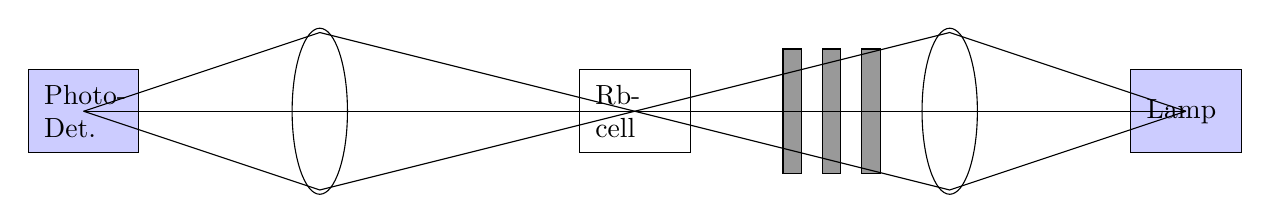
\begin{tikzpicture}
\coordinate (O) at (0,0);
\coordinate (L0) at (-7,0);
\coordinate (L1) at (-4,0);
\coordinate (R0) at (2,0);
\coordinate (R1) at (2.5,0);
\coordinate (R2) at (3,0);
\coordinate (R3) at (4,0);
\coordinate (R4) at (7,0);

\node[block1, name=det] at (L0) {Photo-Det.};
\node[lense, name=lense1] at (L1){};
\node[block2, name=cell] at (O){Rb-cell};
\node[filter, name=f1] at (R0){};
\node[filter, name=f2] at (R1){};
\node[filter, name=f3] at (R2){};
\node[lense, name=lense2] at (R3){};
\node[block1, name=lamp] at (R4){Lamp};
\draw (L0) -- (R4);
\draw (L0) -- (-4,1) -- (4,-1) -- (R4);
\draw (L0) -- (-4,-1) -- (4,1) -- (R4);
\end{tikzpicture}